\documentclass[tikz,border=2pt]{standalone}
\usepackage{amsmath,amssymb}
\usepackage{pgfplots}
\pgfplotsset{compat=1.18}

\begin{document}
% Z ~ N(0,1) and 5 + 2Z ~ N(5,4): scaling by 2 widens the density, shifting by 5 moves it.
% In the MGF the scale enters the argument and the shift gives an exponential factor.
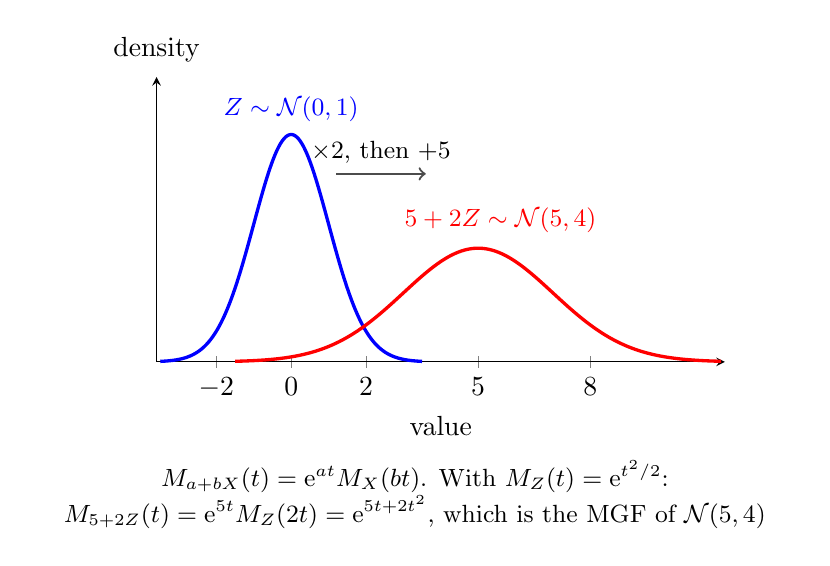
\begin{tikzpicture}
	\begin{axis}[
		axis lines=left, xmin=-3.6, xmax=11.6, ymin=0, ymax=0.5,
		xtick={-2,0,2,5,8}, ytick=\empty,
		xlabel={value}, ylabel={density}, ylabel style={rotate=-90, anchor=south, at={(axis description cs:0,1.02)}},
		samples=160, smooth, width=8.8cm, height=5.2cm, clip=false
		]
		\addplot[blue, very thick, domain=-3.5:3.5] {exp(-x^2/2)/sqrt(2*pi)};
		\addplot[red, very thick, domain=-1.5:11.5] {exp(-(x-5)^2/8)/(2*sqrt(2*pi))};
		\node[blue, anchor=south, font=\small] at (axis cs:0,0.405) {$Z\sim\mathcal{N}(0,1)$};
		\node[red, anchor=south, font=\small] at (axis cs:5.6,0.21) {$5+2Z\sim\mathcal{N}(5,4)$};
		\draw[->, gray!60!black, thick] (axis cs:1.2,0.33) -- (axis cs:3.6,0.33) node[midway, above, font=\small, black] {$\times2$, then $+5$};
	\end{axis}
	\node[anchor=north, font=\small, align=flush center, text width=9.6cm] at ([yshift=-2pt]current axis.outer south) {$M_{a+bX}(t)=\mathrm{e}^{at}M_X(bt)$. With $M_Z(t)=\mathrm{e}^{t^2/2}$: $M_{5+2Z}(t)=\mathrm{e}^{5t}M_Z(2t)=\mathrm{e}^{5t+2t^2}$, which is the MGF of $\mathcal{N}(5,4)$};
\end{tikzpicture}
\end{document}
